\documentclass{article}
% Package and macro definitions for CSC 503
% Originally prepared August 23, 2012 by Jon Doyle

%%% Page dimensions
\setlength{\oddsidemargin}{0in}
\setlength{\evensidemargin}{0in}
\setlength{\topmargin}{0in}
\setlength{\textheight}{9in}
\setlength{\textwidth}{6.5in}
\setlength{\headheight}{0in}
\setlength{\headsep}{0in}
\setlength{\footskip}{0.5in}

%%% Font and symbol definition packages
\usepackage{times} 
\usepackage{helvet} 
\usepackage{alltt}
\usepackage{amsfonts, amsmath}
\usepackage{amssymb}

%%% The modified Sellinger fitch.sty file
\input{fitchhr.sty}

\newcommand{\Z}{\mathbb{Z}}
\newcommand{\Q}{\mathbb{Q}}
\newcommand{\R}{\mathbb{R}}
\newcommand{\N}{\mathbb{N}}
\def\land{\wedge}
\def\lor{\vee}
\def\implies{\rightarrow}
\def\iff{\leftrightarrow}
\def\turn{\vdash}
\def\Cn{\text{Cn}}
\def\Th{\text{Th}}
\def\defeq{\stackrel{\rm def}{=}}

%%% The environment for providing answers to problems
\newenvironment{answer}%
{\par\noindent\textbf{Answer}\par\noindent}%
{}


\usepackage{amsfonts, amsmath, amsthm}
\usepackage{tikz}
\usetikzlibrary{arrows,automata}

\def\Sometime{\mathord{\mathsf{F}}}
\def\Forever{\mathord{\mathsf{G}}}
\def\Next{\mathord{\mathsf{O}}}
\def\NextX{\mathord{\mathsf{X}}}
\def\Until{\mathrel{\mathsf{U}}}
\def\Release{\mathrel{\mathsf{R}}}
\def\WeakUntil{\mathrel{\mathsf{W}}}
\def\Before{\mathrel{\mathsf{B}}}
\def\True{\mathord{\mathsf{true}}}
\def\All{\mathord{\mathsf{A}}}
\def\Exists{\mathord{\mathsf{E}}}
\def\Every{\mathord{\mathsf{E}}}

\title{CSC 503 Homework Assignment 9}
\author{Due October 29, 2014}
\date{October 22, 2014}

\begin{document}
\maketitle

\begin{itemize}
\item \textbf{[40 points total]} Consider the transition model ${\cal
    M}_2$ depicted in Figure \ref{f2} in answering the following
  questions about LTL and CTL statements.
  \begin{figure}[h]
    \centering
    \caption{Model ${\cal M}_2$}
\begin{center}

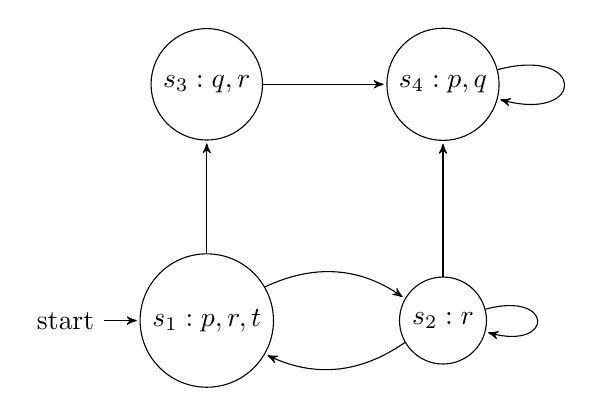
\begin{tikzpicture}[>=stealth',shorten >=1pt,auto,node distance=3cm]
  \node[state] (q3)      {$s_3: q,r$};
  \node[state] (q4)    [right of=q3] {$s_4: p,q$};
  \node[initial,state] (q1)   [below of=q3]   {$s_1: p,r,t$};
  \node[state] (q2)   [right of=q1]   {$s_2: r$};

  \path[->] 
        (q3) edge         node {} (q4)
        (q4) edge [loop right] node {} (q4)
        (q1) edge         node {} (q3)
        (q2) edge         node {} (q4)
        (q2) edge [loop right] node {} (q2)
        (q1) edge    [bend left] node {} (q2)
        (q2) edge    [bend left] node {} (q1);
\end{tikzpicture}
\end{center}
\label{f2}
\end{figure}
  \begin{enumerate}
  \item \textbf{[8 points]} Does ${\cal M}_2, s_4 \models r \implies
    q$?  Explain why or why not.
  \item \textbf{[8 points]} Does ${\cal M}_2, s_1 \models r \implies
    q$?  Explain why or why not.
  \item \textbf{[8 points]} Does ${\cal M}_2, s_3 \models \Sometime
    \neg t$?  Explain why or why not.
  \item \textbf{[8 points]} Does ${\cal M}_2, s_1 \models \Sometime
    \neg t$?  Explain why or why not.
  \item \textbf{[8 points]} Does ${\cal M}_2, s_2 \models \neg \Exists
    \Forever r$?  Explain why or why not.
  \item \textbf{[8 points]} Does ${\cal M}_2, s_4 \models \neg \Exists
    \Forever r$?  Explain why or why not.
  \item \textbf{[8 points]} Does ${\cal M}_2, s_3 \models \Exists
    \Sometime q$?  Explain why or why not.
  \item \textbf{[8 points]} Does ${\cal M}_2, s_1 \models \Exists
    \Sometime q$?  Explain why or why not.
  \item \textbf{[8 points]} Does ${\cal M}_2, s_4 \models \All
    \NextX \All \Forever (p \lor q)$?  Explain why or why not.
  \item \textbf{[8 points]} Does ${\cal M}_2, s_2 \models \All \NextX
    \All \Forever (p \lor q)$?  Explain why or why not.
  \end{enumerate}

%\newpage

\item \textbf{[20 points]} List all subformulas of the CTL formula,
  using Convention 3.13 (p.\ 209) to resolve ambiguities.
  \begin{displaymath}
    \Exists [\All \NextX p \Until (\neg \Exists \NextX q \land \All
    [\neg p \Until \All \Forever (p \lor q)])]
  \end{displaymath}
\end{itemize}

\end{document}
